\documentclass[usenames,dvipsnames]{article}
\usepackage[
		papersize={8in,9in},
		]
	{geometry}
\usepackage{tikz}
  \usetikzlibrary{calc, shapes, backgrounds,angles,quotes,tikzmark}

\usepackage{amssymb} %maths
\usepackage{amsmath} %maths
\usepackage[utf8]{inputenc} %useful to type directly diacritic characters
\usepackage{expex}

\usepackage{ulem}
\begin{document}
	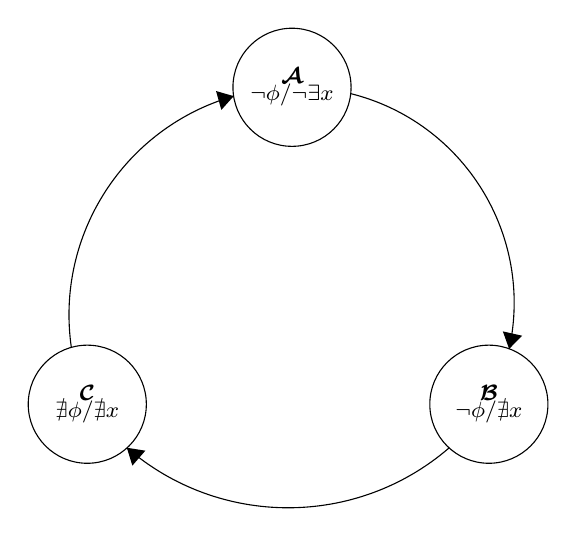
\begin{tikzpicture}[scale=0.25]\footnotesize
	\tikzstyle{every node}+=[inner sep=0pt]
	\draw [black] (23.6,-7.9) circle (3);
	\draw (23.6,-7.9) node[rectangle split,rectangle split parts=2] {$ \boldsymbol{\mathcal{A}} $\nodepart{second} $\neg\phi/\neg\exists x$};
	\draw [black] (13.2,-24) circle (3);
	\draw (13.2,-24) node[rectangle split,rectangle split parts=2] {$ \boldsymbol{\mathcal{C}} $\nodepart{second} $\nexists\phi/\nexists x$};
	\draw [black] (33.6,-24) circle (3);
	\draw (33.6,-24) node[rectangle split,rectangle split parts=2] {$ \boldsymbol{\mathcal{B}} $\nodepart{second} $\neg\phi/\nexists x$};
	\draw [black] (26.574,-8.22) arc (76.02264:-12.33232:10.957);
	\fill [black] (34.63,-21.19) -- (35.29,-20.52) -- (34.31,-20.3);
	\draw [black] (12.391,-21.12) arc (-171.74775:-253.97416:11.563);
	\fill [black] (20.64,-8.35) -- (19.74,-8.09) -- (20.01,-9.05);
	\draw [black] (31.586,-26.214) arc (-49.16439:-130.83561:12.519);
	\fill [black] (15.21,-26.21) -- (15.49,-27.12) -- (16.15,-26.36);
	\end{tikzpicture}
\end{document}